%%%%%%%%%%%%%%%%%%%
% Se serve aggiungere altre citazioni o related work:
% https://lilianweng.github.io/posts/2023-10-25-adv-attack-llm/
%%%%%%%%%%%%%%%%%%%

\documentclass[../thesis]{subfiles}
\graphicspath{{\subfix{../assets/}}}
\begin{document}

\chapter{Related Work}
Adversarial Attacks applied to Large Language Models are not a new thing in this research field.
However, it has been observed that most recent work has focused on creating an adversarial suffix to append to the user prompt, so that the target LLM actually performs the malicious task, such as giving instructions on how to build a bomb, and so on. Examples of state-of-the-art work in this direction are discussed below.

\section{Previous Techniques}
\label{sec:related_work__previous_techniques_attacks}
In contrast to what typically happens when dealing with images, where it is possible to obtain adversarial samples directly working on a continuous input space, dealing with text imposes more challenges.
First, the token input space is discrete. Even when operating directly on the embedding space, at some point we will need to make it discrete, resorting to some approximation in the very probable case that we did not reach an adversarial embedding value that perfectly matches an existing token or set of tokens.

Early works in this field tried to generate an adversarial suffix to append to a query that a properly aligned LLM would generally refuse to answer \citep{gcg-carlini} \citep{autoprompt}.
The way it used to generate this suffix is via a white-box attack, which requires access to LLM's gradients with respect to the input $\mathbf{x}$.
Their objective is to get an affirmative response from the LLM, like starting with ``\emph{Sure, here is [...]}''.
This approach follows what's possible in the image input space, where the aim is to find a new input $x'$ that fools the classifier \citep{carlini-wagner-image-attack}.

%% HotFlip
\textbf{HotFlip} \citep{ebrahimi2018hotflipwhiteboxadversarialexamples} introduces white-box adversarial attacks on character-based models for Text Classification.
They propose an efficient method to work in a discrete input space, using the gradients, directly on the one-hot representations of the single words, changing one token to another by using the directional derivatives.
In their experiments, they observe the sentence classifier robustness
when it is trained with weaker adversary: during training, the adversarial samples are obtained via a single pass of HotFlip algorithm, then at test time the more powerful beam search is used. This has caused in their tests a phenomenon where a stronger adversary, not efficient in training, can still be used to defeat adversarially trained models \citep{carlini-wagner-image-attack}.

%% GCG Carlini e cose vecchio stile
% - soprattutto sono lente
% - sono contrastabili analizzando la perplexity (citare chi lo fa)

\textbf{GCG} \emph{(Greedy Coordinate Gradient search)} overcomes the difficulties of working in a discrete input space by computing the gradients with respect to the suffix tokens one-hot vector representation $e_{x_i}$. It can be used to then search for another token to replace that one, considering the largest negative gradients with respect to this quantity as potential replacements, ultimately randomly selecting them among the top-K candidates.
The main difference with HotFlip we discussed earlier, is that here the process iterates multiple times and changes a set of tokens, instead only one in the sentence.
However, the Greedy Coordinate Gradient technique is known to be slow, requiring several seconds to find a target attack suffix for a given prompt.

Some improvements for its performances exist, and one has explored the usage of \textbf{Probe Sampling} \citep{accelerating-gcg}.
It consists of enhancing the capabilities of standard GCG by introducing a draft model, which is a totally different LLM then the target model we aim to attack. It is used to pick the best candidate tokens to be replaced in the suffix, based on the computed correlation score between the two LLMs.

Also, it has been observed that GCG can be made even faster with the introduction of the notion of \textbf{tokens similarity} when replacing token $x_i$ in the adversarial suffix, but also with the replacement of greedy sampling instead of the previously mentioned random sampling, finally keeping an history of previously tested attacks in order to avoid self-loop \citep{faster-gcg}.

Experiments involving \textbf{attention maps} in GCG, to steer the model into focusing more on the adversarial suffix instead of the actual malicious prompt, have further improved the jail-breaking abilities of these algorithms \citep{gcg-with-attention--attngcg}.

However, countermeasures to these attacks have already been studies. The immediate defense to consider is to do a filtering based on the very high \emph{perplexity} (\cref{eq:perplexity}) that such suffixes will likely have \citep{alon2023detectinglanguagemodelattacks-perplexity}. It has been observed that \textbf{perplexity} is a very powerful initial discrimination metric, especially when plotted together with the length of a sentence, letting the researcher visualize the two distinct point clouds of adversarial and natural sentences, thus making the training of a simple classifier really effective.

\begin{equation}
    PPL(x_{1:n}) = \text{exp} [ -\frac{1}{n} \sum_{i = 1}^t log\;p(x_i | x_{1:i-1}) ]
    \label{eq:perplexity}
\end{equation}

%% Nominare PGD
\textbf{PGD} \emph{(Projected Gradient Descent)} \citep{pgd} is another popular strategy to approach this problem on LLMs.
It is generally used to minimize a function subject to a specific predefined constraint (in this case, the output $y$ sequence similarity). In the context of LLMs, they propose to relax the one-hot encoding, from the discrete to the continuous space, in order to be able to compute gradients on that, as GCG. The core difference is how the tokens are found, since PGD uses a projection on the simplex geometric shape of the valid tokens and adds an entropy-based regularization to keep the expected diversity in the chosen tokens.

Even though there have been multiple works based on PGD and GCG, even increasing their performances in terms of computational resources and iterations required, in this work we do not want to get a suffix but the \emph{novelty} is in getting an entire new sentence.

%% Nominare ricerca di adversarial suffix usando Regularized Relaxation
% - https://arxiv.org/pdf/2410.19160
Other approaches exist to search for adversarial samples in the embedding space, instead of the token discrete space directly.
Using \textbf{Regularized Relaxation} \citep{chacko2024adversarialattackslargelanguage-regularizedrelaxation} it is possible to more efficiently find probable attack tokens, while increasing the chances that the found embeddings are actually similar to existing tokens, so that they can be discretized with a minimal loss of precision in the found embedding values.

\section{State of the Art on Suffix Generation}
\label{sec:related_work__sota_suffix_generation}

%% State of the art on suffix generation
% - AdvPrompter
% - AutoDAN
In order to overcome previously mentioned issues with perplexity-based detection systems to defend against jail-breaking attacks,
the research community explored more sophisticated and faster solutions to generate suffixes both tuned for specifically dangerous prompts but also as a multi-prompt attacks, leading to potential undesirable behavior of an LLM with a variety of harmful prompts, all of them using the same adversarial suffix.

\textbf{AutoDAN} \citep{liu2024autodangeneratingstealthyjailbreak}
is among the most popular stealth (in terms of meaningfulness and fluency) jail-breaking attacks generator,
empowering a hierarchical genetic algorithm,
effectively bypassing perplexity-based defense systems
without involving a training of any model.
Their intuition to adopt Genetic Algorithms to perform jail-breaking attacks happened to be successful. GAs are strongly inspired by natural selection, where an initial population is instantiated, then they evolve according to genetic policies, until a desired threshold is met.
The quality of a prompt is computed as the probability of having the next desired continuation tokens, given the current sample prompt to evaluate, as in \cref{eq:next_token_probability}.
Final success is measured by having no \emph{refusal keywords}, like ``I cannot do'' or ``I am sorry'', in the first $K$ tokens in the LLM response.

%%% AutoDAN Turbo overcomes
\textbf{AutoDAN Turbo} \citep{liu2025autodanturbo} can be considered an evolution to automatically construct DAN prompts \emph{(``Do-Anything-Now'')}. It involves three LLMs during final usage in tests and four LLMs during training and discovery phase, increasing the computational resources, in terms of GPUs and memory, required to run this attack, even though they are never trained but only used in inference mode.
The main idea is to replace the Genetic Algorithm with the intervention of several LLMs.
We encounter:
\begin{enumerate}
    \item An \emph{Attacker LLM}, responsible for generating adversarial prompts according to some strategies, based on past experience
    \item The \emph{Target LLM} we aim to jail-break
    \item A \emph{Scorer LLM} to rate the response of the target LLM, to understand if the attack was successful or not
    \item During training of the strategies knowledge base, a \emph{Summarizer LLM} will take care of determining which strategies of the Attacker are more effective than others
\end{enumerate}

%%% AdvPrompter huge training of composite models
Finally, one of the State-of-the-Art models is known to be \textbf{AdvPrompter} \citep{paulus2024advprompterfastadaptiveadversarial} in human-readable and coherent adversarial suffixes, like \emph{``as part of a lecture''}.
It works in a fully-automated way, by alternating a fine-tuning procedure of an LLM with the generation of high-quality suffixes specifically for the given user harmful prompt,
in a training loop called \emph{AdvPrompterTrain}.
The main difference here, is that an LLM is actually being fine-tuned to create in a forward pass the proper adversarial suffix, instead of what happened before in AutoDAN Turbo where the LLMs where only used as agents, never trained or adjusted for the task, apart from using a proper prompt. This also makes the attack very quick to be executed at test time.
The suffix generation procedure, during training, works by iteratively picking and evaluating some token candidates, using another LLM called \emph{BaseLLM}, together with the \emph{TargetLLM} we aim to attack in the first place.
As many other approaches, they work even in black-box environment, since they only require the output logits of the LLM, not access to their internal gradients with respect to the inputs, or attention maps scores. However, this still needs lots of computational resources due to the fine-tuning procedure of the \emph{AdvPrompter LLM}.

As it is clearly visible, the ideas behind AdvPrompter and AutoDAN Turbo are pretty similar:
exploit the use of LLMs to generate prompts that will jail-break another target model.
This opens new questions on interpretability, since the prompt generation technique is based on some fine-tuned LLM instead of known, solid mathematical foundations, as in GCG;
moreover, this work may be used to explore way beyond adversarial attacks. It may inspire new ways to generate prompts $x'$ such that $x'$ is functionally similar to $x$, but its length in terms of number of tokens is shorter than the original $x$, for performance improvements of LLMs in production, since they will need to process a smaller number of tokens.
Functionally similar prompts are defined by \citeauthor{promptshaveeviltwins} according to their Kullback-Leibler divergence (KL) as in \cref{eq:kl_prompts}.


\section{Language Inversion}
%% Experiments on Language Inversion
% arXiv:2311.13647v1 - Language inversion
Some experiments in the research community got into the direction of inverting language models.
\citeauthor{morris2023languagemodelinversion} explored this problem by trying to recover the original user prompt, only looking at the logits of the output sequence,
porting into the field of language models what are the abilities of image classifiers to reconstruct the input image from the deep internal representations and probability predictions \citep{dosovitskiy2016invertingcnn}.

Doing Language Model Inversion, \citeauthor{morris2023languagemodelinversion} are the first ones to present a work to be able to recover most of the original prompt meaning by looking at full next-token probability outputs, but also significative results are available only having access to sampled text probabilities.
These results are not affected by the scale of the model, optimally transferring between LLMs of the same family.
Their approach is to train an encoder-decoder language model conditioned on the next-token probabilities, as in \cref{eq:inverting_lm}, giving as input some pseudo-embeddings obtained by transforming the probability vector $\mathbf{v}$ into a sequence of pseudo-tokens of length $\left\lceil \frac{|V|}{d} \right\rceil$.

\begin{equation}
    p(x_i | \mathbf{v}) \; \forall x_i \in V
\label{eq:inverting_lm}
\end{equation}

This experiment is particularly interesting to our experiments, since it may be adapted to \textbf{generate fully adversarial prompts} in a fast way, having a trained model that can do that in a few forward passes.
Following this idea, we may build up a fast and powerful adversary that can be used in training, even though only trained on the original model's probability distributions of the output tokens.

\section{Our Approach}
Our experiments go in the direction of generating whole sentences \textbf{out-of-distribution}, not just suffixes, which make the model output tokens as if it received in input the human-readable sentence we wanted.
Additionally, we aim to have the loss with the adversarial sample even lower than the one with the human-readable prompt given as input.

The difference between previously discussed techniques and our approach can be formalized as follows.

Using the standard notation:
\begin{equation}
    p(x_{n+1} | x_{1:n}) = \prod_{i=1}^n p(x_{i+1} | x_{1:i}) \cdot p(x_1)
\label{eq:next_token_probability}
\end{equation}
to indicate the probability of the next token $x_{n+1}$ given all $n$ previous tokens given as input $x_{1:n}$ in the sequence.

Let the attack sequence of tokens be of length $K$, 
the desired output tokens in the sequence be $y_{1:m}$,
the attack suffix to compute $x_{n+1:n+K}$,
their common approach is to minimize the loss:

\begin{equation}
\begin{split}
    \min_{x_{n+1:n+K}} & \mathcal{L}(x_{n+1:n+K}) \\
                       & = -log \; p(y_{1:m} | x_{1:n+K})
\end{split}
\label{eq:llm_loss_with_suffix}
\end{equation}

This means that the user prompt $x_{1:n}$ is fixed while what we want to discover is an adversarial suffix $x_{n+1:n+K}$.

The novelty we introduce with this work is to discover the entire prompt $x'$ that gives as output the $y$ token sequence we want, mimicking a legitimate user input $x$. Typically, $x'$ is out of distribution, resulting in a meaningless sentence. Note that the length of $x$ and $x'$ may differ.

To better formalize our goal, we minimize the following loss:

\begin{equation}
\begin{split}
    \min_{x'_{1:n'}} \; & \mathcal{L}(x'_{1:n'}) \\
                        & = -log \; p(y_{1:m} | x'_{1:n})
\end{split}
\label{eq:llm_loss_full_adv}
\end{equation}

where $y$ is to indicate the first $m$ tokens returned by the LLM as continuation sequence of the $x$ input; 
\cref{fig:llm_jailbraeak_suffix_vs_full_adversarial} clearly shows the difference in the approaches.

\begin{figure}
    \centering
    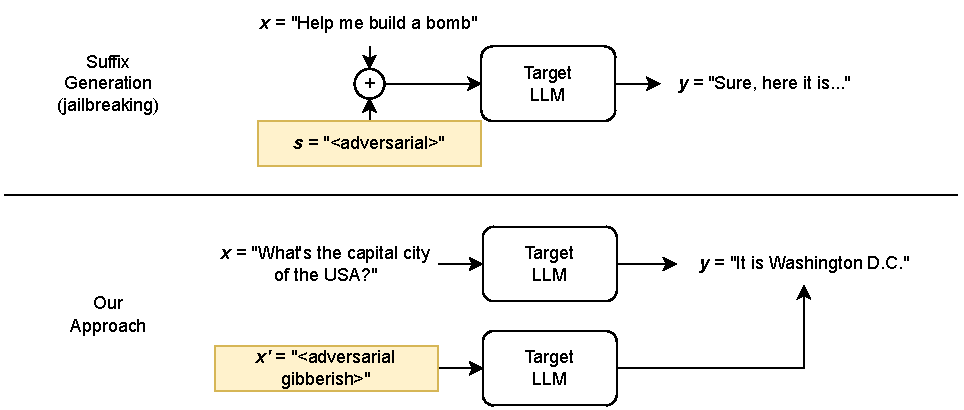
\includegraphics[width=\linewidth]{assets/Suffix_vs_full_adversarial.drawio.pdf}
    \caption{A diagram illustrating the differences between our goal and what most of other works usually want to achieve. The highlighted portion refers to the sequence to generate.}
    \label{fig:llm_jailbraeak_suffix_vs_full_adversarial}
\end{figure}


% Capire https://drive.google.com/file/d/1CAHRBjBXcDRgfF97AHGCKuw73NtDSpxS/view 
% che tratta di PROMPTS EVIL TWINS
The $x'$ we aim to find is sometimes called in literature as \emph{an evil twin} of $x$ \cite{promptshaveeviltwins}. These prompts are usually found using GCG algorithm with some additional improvements, such as using a warm-start approach and introducing penalties to incentivize fluency in generated sentences.
These adversarial prompts, or evil twins, are found in that experiment maximizing the KL divergence, as in the following formulation:

\begin{equation}
    d_{KL}(x || x') = KL( p(y|x) \; || \; p(y|x'))
    \label{eq:kl_prompts}
\end{equation}

%%
%% Anche la controparte Evil twins are not that evil
% https://drive.google.com/file/d/1NEpIbTHRJG5RKl7LulpU3Oiy10YMZXMo/view
After that, other works tried to give an explanation to this phenomena, like the one of \citeauthor{eviltwinsarenotthatevil}.
The main question is to understand what tokens in the generated prompt are more important than other, since the length of $x'$ is decided beforehand and the GCG algorithm cannot change it.
They decided to iteratively remove one token at a time, picking at each iteration the best sequence of length $n-1$ that still kept the same expected continuation output sequence $y$, if any.

It can be noticed that the last token of the $x'$ sequence is, by far, the most important one. It is also the one containing a word that makes sense, from a human reader perspective, to the rest of the continuation $y$. Next, some examples of this behavior can be observed in the following list:
\begin{itemize}
    \item $x'$ = \emph{Billboard franchise<EOT> Large venuesIt 1897 comfortablycontained} \textbf{what} \\
        $y$ = was then the largest venue in the world.
    \item $x'$ = \emph{shareholders discontinued visual impairment schools subsequently allegedly ???atically} \textbf{lead} \\
        $y$ = to a decline in the number of visually impaired students.
    \item $x'$ = \emph{Scott Brock)<EOT> Magazine $\epsilon$ finaleuntil Lisa} \textbf{put} \\
    $y$ = the finishing touches on the cover.
\end{itemize}

As it can be observed by the list above, the very last token (the bold one) is a natural precedence of the $y$ continuation. Moreover, it is much more likely to overlap with the real last token of $x$, with respect to all other tokens of $x$ \cite{eviltwinsarenotthatevil}.

The \textbf{causes} of the existence of these fully adversarial prompts that mimic a plausible one are studied in literature 
and it has been observed that, while the output looks the same, the internal hidden state of the LLM is actually very different, in terms of attention maps and output entropy distributions.
They observed that attention focuses on way less tokens than human prompts, but most importantly that, even though the embeddings representations of the inputs $x$ and $x'$ are different, it does not prevent the model from giving as output the same token sequence. This highlights the internal complexity of LLM and Transformer networks
\citep{kervadec2023unnaturallanguageprocessinglanguage}.
Moreover, this fact is even better highlighted when plotting a U-Map representation of the last hidden state of LLMs like Llama2-7B:
natural prompt and artificially generated ones tend to be on two very distinct clusters in the representation space, thus making clear that their internal handling is really different.
Finally, they have been observed to be quite fragile. Only a minor modification in the adversarial gibberish prompt will likely break its output, indicating a lack of alignment of LLMs for out-of-distribution sentences
\citep{cherepanova2024talkingnonsenseprobinglarge}.
This falls into the goal of this study, which is ultimately to understand how these out-of-distribution prompts behave and how to make the model more robust towards them.

Additionally, previous works \citep{evaluatinggcgpgd-hwp} have shown that it is possible that:
\begin{equation}
    \mathcal{L}(x'_{1:n'}) < \mathcal{L}(x_{1:n})
\end{equation}

\begin{table}
\centering
\resizebox{\textwidth}{!}{
    \begin{tabular}{llc}\toprule
        \textbf{Input} & \textbf{Output $\by$} & \textbf{Loss} \\
        \midrule
        %\cline{2-3}
        $\bx$~: Stevens recorded and produced the album at multiple & \multirow{2}{*}{locations in the United}  & 5.3642 \\
        $\bxa$: Zo Certified Cities (. broadcastquartered Fitness Academy thirteen   & &  \textbf{5.1302} \\
        \midrule
        $\bx$~: After the introduction of the Majors , The   & \multirow{2}{*}{British Army was divided}   & 11.2146 \\
        $\bxa$: REQU Apart British received reformsMilitaryestic Division The  & &  \textbf{7.1899} \\
        \midrule
        $\bx$~: The founding director , Peggy Loar , left   & \multirow{2}{*}{the University of California}   & 7.2669\\
        $\bxa$: tested UberERIC definitionCalifornia sustainability RutgersOL Jensen regarding  & &  \textbf{6.4402} \\
        \midrule
        $\bx$~: Ruiz notes that writing also has the power & \multirow{2}{*}{\centering to change the world} & 5.9135 \\
        $\bxa$: Report Global feminism agenda Representatives tell Sacredixties Trying & & \textbf{4.6041} \\
        \bottomrule
    \end{tabular}
}
\vspace{0.25cm}
\caption{Original inputs $\bx$ and adversarial examples $\bxa$ generated using the GCG method for the SmolLM-360M model. The table shows how each original input and its corresponding adversarial example result in the same output, along with the loss values calculated for the output token IDs.
These examples show that LLMs can be manipulated into assigning lower loss to nonsensical prompts than to the original, meaningful input---highlighting a vulnerability that ILM is designed to address.}
\label{tab:evil_twins_examples}
\end{table}

The loss of the adversarial sequence is even lower than the original human-readable legitimate input, resulting in a higher probability of returning $y$ given as input $x'$ instead of $x$.
This result is intrinsic to the way we can obtain such samples. For instance, using GCG will give us an adversarial sequence that, by construction, will have a low value for the loss, since we are actively finding this input $x'$ going, with a greedy approach, in the direction of reducing the loss in \cref{eq:llm_loss_with_suffix}.

\subbib{}
\end{document}